\section{Лекция 3 (16.09)}
	
\subsection{Двухслойные схемы для нестационарных уравнений}

\subsubsection{Определение}

Рассмотрим дифференциальное уравнение вида

\begin{equation}
    \label{eq:nonstat_common}
    \dfr{u}{t} + Lu = f,
\end{equation}
где $L$ -- произвольный пространственный дифференциальный оператор.
При использовании двухслойной схемы аппроксимации производная по времени записывается в
виде конечной разности с шагом $\tau$, которая может приближать производную
в одном из трёх моментов времени:

\begin{equation}
    \label{eq:nonstat_dt_appr}
    \begin{array}{llll}
        \dfrac{u(t+\tau) - u(t)}{\tau} = 
            & \quad \left.\ddfr{u}{t}\right|_{t}
            & + o(\tau)
            & -\text{ разность вперёд};\\[5pt]
        \phantom{a}
            & \quad \left.\ddfr{u}{t}\right|_{t+\tau}
            & + o(\tau)
            & -\text{ разность назад};\\[5pt]
        \phantom{a}
            & \quad \left.\ddfr{u}{t}\right|_{t+\frac{\tau}{2}}
            & + o(\tau^2)
            & -\text{ симметричная разность.}
    \end{array}
\end{equation}

Момент времени $t$ будем называть текущим временн<strong>ы</strong>м слоем,
момент $t + \tau$ -- следующим,
а момент $t+\tau/2$ -- промежуточным.
Считается, что
значение функции на текущий момент времени $u(t)$ известно, а
значение на следующий момент $u(t+\tau)$ подлежит определению.

\subsubsubsection{Явная схема}

При использовании разности назад уравнение \eqref{eq:nonstat_common}
в полудискретизованном (то есть дискретизованном только по времени, но не по пространству) виде
запишется как
\begin{equation*}
    \frac{u(x, t+\tau) - u(x)}{\tau} + L u(x, t) = f(x, t)
\end{equation*}
или, после переноса всех известных слагаемых вправо
\begin{equation}
    \label{eq:nonstat_explicit}
    u(x, t+\tau) = \left(E - \tau L\right) u(x, t) + \tau f(x, t).
\end{equation}
Здесь $E$ -- единичный оператор.
Схема \eqref{eq:nonstat_explicit} называется явной схемой
и имеет первый порядок точности.

\subsubsubsection{Неявная схема}

Выбрав разность назад из выражения \eqref{eq:nonstat_dt_appr}
полудискретизованная схема для уравнения \eqref{eq:nonstat_common} примет вид
\begin{equation*}
    \frac{u(x, t+\tau) - u(x)}{\tau} + L u(x, t+\tau) = f(x, t+\tau).
\end{equation*}
В результате преобразования получим неявную схему первого порядка точности
\begin{equation}
    \label{eq:nonstat_implicit}
    \left(E+\tau L\right) u(x, t+\tau) = u(x, t) + \tau f(x, t + \tau).
\end{equation}

\subsubsubsection{Схема Кранка--Николсон}

Подставим симметричную разность из \eqref{eq:nonstat_dt_appr}
в уравнение \eqref{eq:nonstat_common}. Формально получим
\begin{equation*}
    \frac{u(x, t+\tau) - u(x)}{\tau} + L u(x, t+\frac{\tau}{2}) = f(x, t+\frac{\tau}{2}).
\end{equation*}

Для определения выражения функций на промежуточном временном слое
распишем значение $u$ на текущем и следующем слоях в ряд Тейлора
относительно значения на момент $t+\tau/2$:
\begin{align*}
    u\left(t\right)      &= u\left(t+\frac{\tau}{2}\right) - \left.\frac{\tau}{2}\dfr{u}{t}\right|_{t+\frac{\tau}{2}} + o(\tau^2)\\
    u\left(t+\tau\right) &= u\left(t+\frac{\tau}{2}\right) + \left.\frac{\tau}{2}\dfr{u}{t}\right|_{t+\frac{\tau}{2}} + o(\tau^2)
\end{align*}
Взяв полусумму этих выражений получим аппроксимацию функции на промежуточном слое:
\begin{equation}
    \label{eq:nonstat_cn_appr}
    u\left(x, t + \frac{\tau}{2}\right) = \frac12u\left(x, t\right) + \frac12u\left(x, t+\tau\right) + o(\tau^2)
\end{equation}
Аналогичная запись справедлива и для свободного члена $f$.
Если оператор $L$ -- нестационарный или нелининый, то аппроксимацию \eqref{eq:nonstat_cn_appr}
следует записывать для всего выражения $Lu$:
\begin{equation*}
    \left(Lu\right)_{t+\frac{\tau}{2}} = \frac12\left(Lu\right)_{t} + \frac12\left(Lu\right)_{t+\tau} + o(\tau^2)
\end{equation*}


С учётом \eqref{eq:nonstat_cn_appr} симметричная разностная схема
запишется как
\begin{equation*}
    \frac{u(x, t+\tau) - u(x)}{\tau} + \frac12L u(x, t) + \frac12 L u(x, t + \tau) = \frac12 f(x, t) + \frac12 f(x, t+\tau)
\end{equation*}
или
\begin{equation}
    \label{eq:nonstat_cn}
    \left(E+\frac{\tau}{2} L\right) u(x, t+\tau) = \left(E - \frac{\tau}{2} L\right) u(x, t) + \frac{\tau}{2} \left(f(x, t) + f(x, t + \tau)\right).
\end{equation}
Такая схема называется схемой Кранка--Николсон и имеет второй порядок аппроксимации по времени.

В случае, если оператор $L$ зависит от времени, то
в левой части схемы \eqref{eq:nonstat_cn} его нужно
брать на следующем временном слое, а в правой -- на текущем.

\subsubsubsection{Обобщённая двухслойная схема}

Выражения
\eqref{eq:nonstat_explicit},
\eqref{eq:nonstat_implicit},
\eqref{eq:nonstat_cn}
можно записать в обобщённой форме
\begin{equation}
    \label{eq:nonstat_theta}
    \left(E+\theta\tau L\right) u(x, t+\tau) = \left(E + \left(\theta - 1\right)\tau L\right) u(x, t) + \left(1 - \theta\right) f(x, t) + \theta f(x, t + \tau).
\end{equation}
Коэффициент $\theta$ -- степень неявности схемы:
\begin{itemize}
\item $\theta = 0$ -- явная схема \eqref{eq:nonstat_explicit},
\item $\theta = 1$ -- полностью неявная схема \eqref{eq:nonstat_implicit},
\item $\theta = 1/2$ -- схема Кранка--Николсон \eqref{eq:nonstat_cn}.
\end{itemize}

Отметим, что только при $\theta = 1/2$ схема \eqref{eq:nonstat_theta} имеет второй порядок точности по времени.
Для других значений (в том числе промежуточных) схема будет иметь ошибку первого порядка $o(\tau)$.

\subsubsection{Дискретизация по времени как итерационный процесс}

\subsubsubsection{Двухслойный итерационный процесс}

Простой двухслойный итерационный процесс определяется как
\begin{equation}
    \label{eq:nonstat_common_iter}
    u^{n+1} = A u^{n} + b,
\end{equation}
где $n$ -- индекс итерационного слоя,
$A$ -- оператор преобразования,
$b$ -- свободный член.

Определение значения функции на следующий момент времени $u(t+\tau)$ 
по двухслойной схеме \eqref{eq:nonstat_theta} можно представить как простой итерационный процесс \eqref{eq:nonstat_common_iter}, где
\begin{align*}
    A &= \left(E + \theta \tau L \right)^{-1} \left(E + (\theta - 1) \tau L \right), \\\\
    b &= \left(E + \theta \tau L \right)^{-1} \left( \theta f\left(x, t + \tau\right) + \left(1 - \theta\right) f\left(x, t\right) \right).
\end{align*}

Итерационный процесс называется сходящимся, если
\begin{equation*}
    \lim_{n=\infty} \left\lVert u^{n+1} - u^{n} \right\rVert = 0.
\end{equation*}

\subsubsubsection{Устойчивость итерационного процесса}
\label{sec:ScalarIter}

Рассмотрим два простых итерационных процесса,
имеющих на нулевом слое значение $u^0 = 1$:
\begin{align*}
    {\rm (I)}:\quad  &u^{n+1} = 2 u^{n} - 1, \\
    {\rm (II)} :\quad  &u^{n+1} = 0.5 u^{n} + 0.5.
\end{align*}
Оба этих процесса при выбранном начальном приближении, очевидно, сходятся.
На каждой итерации справделиво $u^n = 1$.
Возмутим начальное условие: пусть
\begin{equation*}
    u^0 = 1 + \eps,
\end{equation*}
и проведём итерации.
\begin{equation*}
    \def\arraystretch{1.7}
    \begin{array}{c|c|c}
        & {\rm (I)}  &  {\rm (II)} \\
        \hline
        u^1 & 1 + 2\eps & 1 + \dfrac{\eps}{2} \\
        \hline
        u^2 & 1 + 4\eps & 1 + \dfrac{\eps}{4} \\
        \hline
        u^3 & 1 + 8\eps & 1 + \dfrac{\eps}{8} \\
        \hline
        ... & & \\
        \hline
        u^\infty & \infty & 1 \\
    \end{array}
\end{equation*}

Видно, что процесс $\rm (I)$ теряет сходимость и стремится к бесконечности,
в то время, как процесс $\rm (II)$ сохраняет свои свойства.

Свойство итерационных процессов уменьшать малые возмущения называется устойчивостью.
В примере выше процесс $\rm (I)$ является неустойчивым, а процесс $\rm (II)$ -- устойчивым.

Нетрудно видеть, что для рассматриваемого скалярного итерационного процесса,
условие устойчивости запишется в виде $|A| \leq 1$.

\subsubsubsection{Источники возмущений}

На практике возникновение возмущений в решениях неизбежно:
они могут быть следствием ошибок дискретизации функций и операторов,
погрешностей решения СЛАУ, ошибок при проведении арифметических
операций на числах с плавающей точкой и т.д.
Поэтому любой итерационный процесс, используемый для решений
математических задач, должен быть устойчив.

Возникновение непреднамеренных ошибок вследствии компьютерного округления можно проиллюстрировать на примере
программы, в которой рассматривается сходящийся для любого начального условия, но неустойчивый итерационный процесс
\begin{equation*}
    u^{n+1} = 10 u^{n} - 9 u^{0}.
\end{equation*}

\begin{minted}[linenos=false]{c++}
double u0 = 0.625;
double u = u0;
for (int i=0; i<1000; ++i){
    u = 10*u - 9*u0;
}
std::cout << u << std::endl;
\end{minted}

Если начальное значение может быть точно представлено в
числах с плавающей точкой (путём конечной суммы степеней двойки),
то арифметическая ошибка не возникает.
Так, представленный выше код на выходе печатает ожидаемое $u=0.625$.
Потому что начальное приближение может быть разложено как $u^0 = 2^{-1} + 2^{-3}$.

Однако, если заменить начальное приближение на любое число,
которое не может быть записано точно во floating-point формате,
то процесс быстро уходит в бесконечность.
Например, для $u^0 = 0.626$ бесконечные (непредставимые в машинном формате) значения
появляются на 324-ой итерации,
а при переключении на работу в числах одинарной точности `float` -- уже на 46-ой.

\subsection{Методы исследования устойчивости расчётных схем}
\label{sec:stability_analysis}

\subsubsection{Матричный метод}

Итерационные процессы, возникающие при численном решении
дифференциальных уравнений сеточными методами, имеют матричную природу.
То есть оператор преобразования $A$ в выражении \eqref{eq:nonstat_common_iter} -- это матрица,
а функции $u$ и $b$ -- векторы-столбцы.

Как было показано выше, условием устойчивости скалярного итерационного процесса является неравенство $|A| \leq 1$.
Аналогом этого условия для матричного процесса является ограничение на спектральный радиус $S(A)$:
\begin{equation}
    \label{eq:nonstat_spectral_radius}
    S(A) = \max_j{ | \lambda_j | } \leq 1,
\end{equation}
где $\lambda_j$ -- собственные числа матрицы $A$.

Для некоторых видов матриц, возникающих при аппроксимации простейших дифференциальных уравнений,
собственные числа известны.

\subsubsubsection{Явная схема для нестационарного уравнения диффузии}
\label{sec:NonstatExpDiff}

Например, рассмотрим одномерное нестационарное уравнение диффузии с граничными условиями первого рода
\begin{align*}
    &\dfr{u}{t} = k\dfrq{u}{x},\\[5pt]
    &u(x, 0) = u_0(x),\\[5pt]
    &u(x_a, t) = u_a,\\[5pt]
    &u(x_b, t) = u_b.\\
\end{align*}
Используем явную дискретизацию по времени и аппроксимацию второго порядка по пространству.
Тогда разностная схема запишется в виде:
\begin{equation}
    \label{eq:nonstat_explicit_diff}
    \hat u_i = u_i + \gamma (u_{i-1} - 2 u_i + u_{i+1}), \quad i = \overline{1, N-1},
\end{equation}
где введено обозначение для значения функции на следующем временном слое $\hat u = u(t+\tau)$ и $\gamma = \tau k / h^2 $.
В матричном виде схема имеет вид
\begin{equation*}
    \hat u = A u, \quad
    A = \left(
        \begin{array}{cccccc}
            1      & 0          &           &            &           &        \\
            \gamma & 1-2\gamma  & \gamma    &            &           &        \\
                   & \gamma     & 1-2\gamma & \gamma     &           &        \\
                   &            & \ddots    & \ddots     & \ddots    &        \\
                   &            &           & \gamma     & 1-2\gamma & \gamma \\ 
                   &            &           &            & 0         & 1      
        \end{array}
    \right).
\end{equation*}
Первая и последняя строки этой матрицы -- следствие учёта граничных условий первого рода.

Собственные числа для полученной трёхдиагональной матрицы преобразования в правой части имеют вид
\begin{equation*}
    \lambda_j = 1 - 4\gamma\sin^2\left(\frac{j\pi}{2 N}\right), \quad j = \overline{1, N-1}
\end{equation*}
Тогда, исходя из выражения \eqref{eq:nonstat_spectral_radius}, запишем условие устойчивости
для явной схемы \eqref{eq:nonstat_explicit_diff}
\begin{equation*}
    \gamma \leq \frac12
\end{equation*}

\subsubsubsection{Неявная схема для нестационарного уравнения диффузии}\
\label{sec:NonstatImpDiff}

Аналогично, рассмотрим неявную схему
\begin{equation}
    \label{eq:nonstat_implicit_diff}
    \hat u_i - \gamma (\hat u_{i-1} - 2 \hat u_i + \hat u_{i+1}) = u_i, \quad i = \overline{1, N-1},
\end{equation}
В матричном виде
\begin{equation*}
    \hat u = A^{-1} u, \quad
    A = \left(
        \begin{array}{cccccc}
            1      & 0          &           &            &           &        \\
            -\gamma& 1+2\gamma  &-\gamma    &            &           &        \\
                   &-\gamma     & 1+2\gamma &-\gamma     &           &        \\
                   &            & \ddots    & \ddots     & \ddots    &        \\
                   &            &           &-\gamma     & 1+2\gamma &-\gamma \\ 
                   &            &           &            & 0         & 1      
        \end{array}
    \right).
\end{equation*}

Собственные числа такой матрицы имеют вид
\begin{equation*}
    \lambda_j = 1 + 4\gamma\sin^2\left(\frac{j\pi}{2 N}\right), \quad j = \overline{1, N-1}
\end{equation*}
Поскольку в правой части итерационного процесса используется матрица, обратная к $A$,
а собственные числа обратных матриц равны $1/\lambda_j$, то условие устойчивости
примет вид
\begin{equation*}
    \lambda_j \geq 1.
\end{equation*}
Очевидно, что оно выполняется всегда. Поэтому неявная схема \eqref{eq:nonstat_implicit_diff} безусловно устойчива.

\subsubsection{Метод дискретных возмущений}

Метод дискретных возмущений заключается
в использовании в качестве начального приближения
нулевого вектора, с возмущением $\eps$
в одном из узлов:
\begin{equation*}
    u^0 = \left(
        \begin{array}{c}
            0\\
            \vdots\\
            0\\
            \eps\\
            0\\
            \vdots\\
            0
        \end{array}
        \right)
\end{equation*}
и дальнейшем анализом
распространения этого возмущения с прохождением
по временным слоям.
Во многом этот метод аналогичен тому алгоритму,
по которому мы иллюстрировали устойчивость
простейшего скалярного итерационного процесса (\ref{sec:ScalarIter}).

\subsubsubsection{Явная схема против потока для уравнения переноса}
\label{sec:NonstatExpTran}

Для иллюстрации рассмотрим одномерное уравнение переноса
\begin{equation}
    \label{eq:nonstat_transport}
    \dfr{u}{t} + V\dfr{u}{x} = 0
\end{equation}
и явную противопоточную схему для него (при условии $V > 0$)
\begin{equation}
    \label{eq:nonstat_explicit_transport}
    \hat u_i = u_i - C \left(u_i - u_{i-1}\right),
\end{equation}
где число Куранта определено как $C = \tau V /h $.

Пусть $u_i = \eps$. Тогда
\begin{align*}
    & \hat u_i = (1 - C) \eps & \hence & \; 0 \leq C \leq 2,  \\[5pt]
    & \hat u_{i+1} = C \eps   & \hence & \; -1 \leq C \leq 1.
\end{align*}
Поскольку $C$ по определению больше нуля, то условием устойчивости для схемы $\eqref{eq:nonstat_explicit_transport}$
будет выражение
\begin{equation*}
    C \leq 1.
\end{equation*}

\subsubsection{Метод Неймана}

Запишем обратное преобразование Фурье для функции u(x):
\begin{equation*}
    u(x) = \int v(\kappa) e^{\imi \kappa x} \, d\kappa,
\end{equation*}
$\kappa$ -- волновое число, $\imi$ -- мнимая единица, $v(\kappa)$ -- Фурье образ исходной функции.

Зададим такое начальное возмущение, которое имеет единичную амплитуду 
на одной частоте, соответствующей волновому числу $\kappa_0$:
\begin{equation*}
    v(\kappa) = \delta(\kappa - \kappa_0),
\end{equation*}
$\delta(x)$ -- функция Дирака.
Кроме того, учтём, что $x_i = ih$.
Тогда выбранное начальное возмущение на одной выбранной частоте, взятое в $i$-ом узле, примет вид
\begin{equation}
    \label{eq:nonstat_neumann_decomp}
    u_i = e^{\imi i \theta}, \quad \theta = \kappa_0 h
\end{equation}
На следующем временном шаге это возмущение примет вид:
\begin{equation}
    \label{eq:nonstat_neumann_decomp_hat}
    \hat u_i = G e^{\imi i \theta}.
\end{equation}
$G$ -- коэффициент усиления. Он показывает во сколько раз
увеличилась амплитуда выбранного возмущения за один шаг по времени.
Для того, чтобы все возмущения затухали, необходимо
\begin{equation*}
    |G| \leq 1, \quad \forall \theta
\end{equation*}

\subsubsubsection{Неявная противопотоковая схема для уравнения переноса}
\label{sec:NonstatImpConv}

Для примера анализа устойчивости методом Неймана опять рассмотрим задачу $\eqref{eq:nonstat_transport}$,
но на этот раз рассмотрим чисто неявную аппроксимацию
\begin{equation}
    \label{eq:nonstat_implicit_transport}
    \hat u_i + C \left(\hat u_i - \hat u_{i-1}\right) = u_i.
\end{equation}

Подставим $\eqref{eq:nonstat_neumann_decomp}$, $\eqref{eq:nonstat_neumann_decomp_hat}$
\begin{equation*}
    G e(i) + C \left(G e(i) - G e(i-1)\right)= e(i). 
\end{equation*}
где для краткости введено обозначение
\begin{equation*}
    e(i) = e^{\imi \theta i}.
\end{equation*}
Поделим на $e(i)$ с использованием свойств этой степенной функции. Тогда

\begin{align*}
    & G + C G \left(1 - e(-1)\right)= 1 \quad \hence \\[10pt]
    & G = (1 + C (1 - e(-1)))^{-1}.
\end{align*}
По определению комплексной экспоненты имеем
\begin{equation*}
    e(-1) = \cos \theta - \imi \sin\theta.
\end{equation*}
Требуется показать, что $|G| \leq 1$. Отсюда
\begin{align*}
    & |1 + C (1 - \cos\theta + \imi\sin\theta)|  \geq 1 \quad \hence \\[10pt]
    & |1 + C (1 - \cos\theta) + C\imi\sin\theta)|^2 \geq 1 \quad \hence \\[10pt]
    & 1 + C^2(1-\cos\theta)^2 + 2C(1-\cos\theta) + C^2\sin^2\theta \geq 1 \quad \hence \\[10pt]
    & C^2(1-\cos\theta) + 2C + C^2(1+\cos\theta) \geq 0 \quad \hence \\[10pt]
    & C^2 + 2C \geq 0.
\end{align*}
По определению число Куранта больше 0, поэтому последнее выражение выполняется всегда.
Отсюда следует вывод, что неявная разностная схема вида $\eqref{eq:nonstat_implicit_transport}$
безусловно устойчива.

\subsubsubsection{Противопотоковая схема Кранка-Николсон для уравнения переноса}
\label{sec:NonstatCNConv}

Для того же самого уравнения $\eqref{eq:nonstat_transport}$
рассмотрим схему Кранка-Николсон $\eqref{eq:nonstat_cn_appr}$:
\begin{equation}
    \label{eq:nonstat_cn_transport}
    \hat u_i + \frac{C}{2} \left(\hat u_i - \hat u_{i-1}\right) = u_i - \frac{C}{2} \left(u_i - u_{i-1}\right).
\end{equation}
Так же
подставим $\eqref{eq:nonstat_neumann_decomp}$, $\eqref{eq:nonstat_neumann_decomp_hat}$
и поделим на $e(i)$:
\begin{align*}
    & G + \frac{C G}{2} \left(1 - e(-1)\right) = 1 - \frac{C}{2} \left(1 - e(-1)\right) \quad \hence \\[10pt]
    & G = \frac{1 - p}{1 + p}, \quad p = \frac{C}{2} \left(1 - e(-1)\right).
\end{align*}
Для выполнения условия устойчивости $|G| \leq 1$, необходимо
\begin{align*}
    & |1-p|^2 \leq |1+p|^2 \quad \hence \\[10pt]
    & (1 - \Re(p))^2 + \Im(p)^2 \leq (1+\Re(p))^2 + \Im(p)^2  \quad \hence \\[10pt]
    & \Re(p) \geq 0
\end{align*}
Здесь $\Re(p)$, $\Im(p)$ -- дейсвительная и мнимая часть комплексного числа.

Поскольку число Куранта больше нуля, то и действительная часть выражения $p$ неотрицательная для любого $\theta$.
\begin{equation*}
    \Re(p) = \frac{C}{2} \left(1 - \cos\theta\right) \geq 0.
\end{equation*}
Получаем, что схема видеа $\eqref{eq:nonstat_cn_transport}$ безусловно устойчива.

\subsubsubsection{Явная схема для уравнения нестационарной конвекции-диффузии}
\label{sec:NonstatExpConvDiff}

Рассмотрим уравнение конвекции-диффузии
\begin{equation}
    \label{eq:nonstat_convdiff}
    \dfr{u}{t} + V\dfr{u}{x} = k\dfrq{u}{x}
\end{equation}

Сначала напишем чисто явную схему второго порядка по пространству:
\begin{equation}
    \label{eq:nonstat_convdiff_explicit}
    \frac{\hat u_i - u_i}{\tau} + V\frac{u_{i+1} - u_{i-1}}{2h} = k\frac{u_{i+1} - 2 u_{i} + u_{i-1}}{h^2}
\end{equation}
Введем число Куранта $C = V \tau/h$ и параметр $\gamma = k \tau / h^2$. Тогда

\begin{equation*}
    \hat u_i = \left(\gamma - \frac{C}{2}\right) u_{i+1} + \left(\gamma + \frac{C}{2}\right) u_{i-1} + (1 - 2\gamma) u_i.
\end{equation*}
Далее подставим $\eqref{eq:nonstat_neumann_decomp}$, $\eqref{eq:nonstat_neumann_decomp_hat}$
\begin{equation*}
    G e(i) = \left(\gamma - \frac{C}{2}\right) e(i+1) + \left(\gamma + \frac{C}{2}\right) e(i-1) + (1 - 2\gamma) e(i).
\end{equation*}
Поделим на $e(i)$ с использованием свойств этой степенной функции. Тогда
\begin{equation*}
    G = \gamma(e(1) + e(-1)) - \frac {C}{2} (e(1) - e(-1)) + (1 - 2\gamma)
\end{equation*}
По определению комплексной экспоненты имеем
\begin{align*}
    e(1) &= \cos \theta + \imi \sin\theta,\\
    e(-1) &= \cos \theta - \imi \sin\theta,
\end{align*}
Отсюда
\begin{equation*}
    G = 2\gamma\cos\theta - \imi {C} \sin\theta + (1 - 2\gamma)
\end{equation*}
Запишем квадрат модуля комплексного числа $G$:
\begin{align*}
    |G|^2 = & \left(1 - 2\gamma(1-\cos\theta)\right)^2 + C^2 \sin^2\theta =\\
            & 1 + 4 \gamma^2(1-\cos\theta)^2 - 4\gamma(1-\cos\theta) + C^2 (1 - \cos^2\theta).
\end{align*}

Требование $|G| \leq 1$ эквивалентно $|G|^2 \leq 1$, или
\begin{align*}
    &1 + 4 \gamma^2(1-\cos\theta)^2 - 4\gamma(1-\cos\theta) + C^2 (1 - \cos^2\theta) \leq 1 \quad \hence \\[5pt]
    &4 \gamma^2(1-\cos\theta)^2 - 4\gamma(1-\cos\theta) + C^2 (1 - \cos^2\theta) \leq 0 \quad \hence \\[5pt]
    &4 \gamma^2(1-\cos\theta) - 4\gamma + C^2 (1 + \cos\theta) \leq 0 \quad \hence \\[5pt]
    &(C^2 - 4 \gamma^2) \cos\theta +4\gamma^2 - 4\gamma + C^2 \leq 0
\end{align*}

Поскольку неравенство должно выполняться для всех $\theta$,
а полученное выражение линейно зависит от $\cos\theta$, то будет достаточно рассмотреть два экстремальных значения косинуса,
из которых окончательно запишем два условия устойчивости для явной дискретизации уравнения конвекции-диффузии вида \eqref{eq:nonstat_convdiff_explicit}:
\begin{equation}
    \label{eq:nonstat_convdiff_explicit_cond}
    \begin{array}{lcl}
        \cos\theta = 1  & \hence & C \leq \sqrt{2\gamma}, \\
        \cos\theta = -1 & \hence & \gamma \leq 1/2.
    \end{array}
\end{equation}

Обычно вместо первого из условий \eqref{eq:nonstat_convdiff_explicit_cond} применяют
более жёсткое (в случае $2\gamma < 1$) условие
\begin{equation*}
    C \leq 2\gamma,
\end{equation*}
которое с учётом определений сводится к условию на шаг по пространству, формулируемому в терминах сеточного числа Рейнольдса $\Ren_c$:
\begin{equation*}
    \frac{V h}{k} \equiv \Ren_c \leq 2.
\end{equation*}

\subsubsubsection{Неявная схема для уравнения нестационарной конвекции-диффузии}
\label{sec:NonstatImpConvDiff}

Аналогичным образом рассмотрим неявную диффузии схему для уравнения \eqref{eq:nonstat_convdiff} вида
\begin{equation}
    \label{eq:nonstat_convdiff_semi_implicit}
    \frac{ \hat u_i - u_i}{\tau} + V\frac{ u_{i+1} - u_{i-1}}{2h} = k\frac{\hat u_{i+1} - 2 \hat u_{i} + \hat u_{i-1}}{h^2}
\end{equation}

Подставляя представление для возмущения с волновым числом $\theta$, получим
\begin{equation*}
    G = \frac{1 - \imi C \sin\theta}{1 - 2\gamma(\cos\theta - 1)}
\end{equation*}

Для устойчивости необходимо
\begin{align*}
    & |1 - \imi C \sin\theta|^2 \leq |1 - 2\gamma(\cos\theta - 1)|^2 \quad \hence \\[10pt]
    & 1 + C^2\sin^2\theta \leq 1 + 4\gamma^2(1 - \cos\theta)^2 + 4\gamma(1-\cos\theta) \quad \hence \\[10pt]
    & C^2(1 + \cos\theta) \leq 4\gamma^2(1 - \cos\theta) + 4\gamma \quad \hence \\[10pt]
    & \cos\theta(C^2 + 4\gamma^2) + C^2 - 4\gamma - 4\gamma^2 \leq 0
\end{align*}
Наибольшего значения выражение слева достигает при $\theta = 0$. Тогда единственное условие устойчивости 
примет вид
\begin{equation*}
    C \leq \sqrt{2\gamma}.
\end{equation*}

\subsubsection{Общие рекомендации к выбору устойчивых расчётных схем}
Теоретический анализ условий устойчивости возможен
лишь для простейших уравнений с постоянными шагами дискретизации.
В практических приложениях, имеющих дело, как правило,
с неструктурированными сетками и сложными нелинейными системами уравнений,
параметры устойчивого счёта приходится определять эмпирически.
Однако, такой теоретический анализ позволяет выделить принципы, которыми
следует руководствоваться для построения устойчивых схем.

{\bf Неявные схемы более устойчивы, чем явные}
\begin{itemize}
\item
Это можно видеть, сравнив результаты анализа
для безусловно устойчивой неявной схемы (\ref{sec:NonstatImpDiff}) для уравнения диффузного переноса и
для условно устойчивой явной схемы (\ref{sec:NonstatExpDiff}).
\item
Для уравнения переноса с разностью против потока
явная (\ref{sec:NonstatExpTran}) схема условно устойчива, в то время как
неявная (\ref{sec:NonstatImpConv}) -- устойчива безусловно.
\item
Даже если только часть схемы неявная, это повышает устойчивость.
Так,  явная (\ref{sec:NonstatExpConvDiff}) схема для уравнения конвекции-диффузии
имеет два условия устойчивости, в то время как
схема, неявная по диффузии (\ref{sec:NonstatImpConvDiff}) -- только одно.
\item
Аналогично,  явная (\ref{sec:NonstatExpTran}) схема против потока для
уравнения переноса условно устойчива,
а схема Кранка-Николсон (\ref{sec:NonstatCNConv}) для того же уравнения устойчива при любых параметрах.
\end{itemize}

{\bf Конвективное слагаемое провоцирует неусточивость, а диффузионное -- напротив, добавляет устойчивость}
\begin{itemize}
\item
Так, схемы с центральными разностями для уравнения конвекции-диффузии
(и явная (\ref{sec:NonstatExpConvDiff}), и полунеявная (\ref{sec:NonstatImpConvDiff})),
условно устойчивы. Явная схема с центральными разностями для чистого уравнения переноса всегда неустойчива.
В последнем можно убедится, подставив $k=0$ в условия устойчивости для уравнений конвекции-диффузии.
\end{itemize}

\subsection{Программная реализация схемы для уравнения переноса}

\subsubsection{Постановка задачи}
Рассматриваются три схемы по времени для противопотоковой аппроксимации уравнения переноса \eqref{eq:nonstat_transport}: 
\begin{itemize}
\item явная схема \eqref{eq:nonstat_explicit_transport} (тест называется \cvar{[transport1-explicit]}),
\item неявная схема \eqref{eq:nonstat_implicit_transport} (\cvar{[transport1-implicit]}),
\item схема Кранка--Николсон \eqref{eq:nonstat_cn_transport} (\cvar{[tranport1-cn]}).
\end{itemize}

Уравнение решается на отрезке $x\in[0, 1]$ с единичной скоростью $V = 1$
на сетке из 1000 ячеек. Временные итерации продолжаются до момента времени $t = 0.5$.

Начальным условием является функция вида
\begin{equation*}
    u(x, 0) = e^{-x^2/\sigma^2}, \quad \sigma = 0.1
\end{equation*}
Точное решение уравнения, с которого будут сниматься граничные условия и производится сравнения полученного численного решения,
запишется как
\begin{equation*}
    u(x, t) = u(x - t, 0) = e^{-(x-t)^2/\sigma^2}.
\end{equation*}

На каждом шаге по времени функция сохраняется в vtk-формате.
В конце выводится значение отклонения от точного решения на конечный момент времени.

В качестве цели решения обозначим построение решения и визуальное сравнение решений
при числе $C=0.9$ по трём разным схемам.
А также построение графика сходимости отклонения точного решения
от численного при изменении числа Куранта и фиксированном шаге по пространству
(то есть сходимость при уменьшении шага по времени).

Программы реализованы в файле \ename{transport_solve_test.cpp}.
\clisting{open}{"test/transport_solve_test.cpp"}

\subsubsection{Функция верхнего уровня}

Для всех трёх программ функция верхнего уровня имеет один и тот же вид.
Рассмотрим на примере первой из них:
\clisting{line}{"[transport1-explicit]"}

В начале происходит установка параметров численной схемы:
\begin{itemize}
\item конечного момента времени,
\item скорости переноса,
\item длины расчётной области,
\item разбиения по пространству,
\item числа Куранта
\end{itemize}

\clisting{lines-range}{"const double", "Cu"}

Далее вычисляются используемые шаги:
\begin{itemize}
\item шаг по пространству (из длины области и разбиения),
\item шаг по времени (из шага по пространству и числа Куранта)
\end{itemize}

\clisting{lines-range}{"double h", "double tau"}

Потом устанавливается рабочий класс, в котором будет производится решение
\clisting{line}{"TestTransport1WorkerExplicit worker"}

Конструируется класс, используемый для связного сохранения
полей на разные моменты времени.
Этот класс создаёт \ename{transport1-explicit.vtk.series}
со списком всех сохранённых полей и отнесёнными к ним моментами времени,
который можно впоследствии открыть в Paraview и использовать
функции анимации для воспроизведения поведения решения во времени.
\clisting{line}{"VtkUtils::TimeSeriesWriter writer(\"transport1-explicit\");"}
Далее нужно в этот класс сохранить решение на начальный момент времени.
Для этого туда сначала добавляется запись о нулевом моменте времени
\clisting{line}{"out_filename"}
В переменную \cvar{out_filename} записывается конкретное
имя vtk-файла, куда следует сохранить решение.
Уже это имя используется для сохранения решения на текущий (начальный) момент времени.
\clisting{line}{"out_filename"}

Далее начинается цикл по времени,
продолжающийся до тех пор, пока внутреннее время решателя
не достигнет конечного
\clisting{line}{"while"}

Внутри вызывается функция решения, которая продвигает
внутреннее время решателя на $\tau$, обновляет
актуальное состояние вектора решения
и возвращает текущую норму.
\clisting{line}{"norm"}

Потом повторяется процедура сохранения
текущего состояния решателя
\clisting{lines-range}{"out_filename", "save_vtk"}

После завершения цикла в консоль печатается
установленное разбиение по времени и
полученное отклонение от точного решения
на конечный момент времени 
\clisting{line}{"cout"}

\subsubsection{Расчётные функции}

Три класса-решателя для трёх заявленных задач:
\cvar{TestTransport1WorkerExplicit},
\cvar{TestTransport1WorkerImplicit},
\cvar{TestTransport1WorkerCN}
наследуются от одного абстрактного класса
\cvar{ATestTransport1Worker}. В этом
абстрактном классе реализованы
все общие для всех решателей функции:
создание сетки, сохранение в vtk,
расчёт нормы, продвижение по времени.

Этот класс также хранит в себе параметры, полностью определяющие текущее состояние решения:
\begin{itemize}
\item расчётную сетку,
\item шаг по времени (это параметр, производный от сетки, он сохранён в отдельное поле для удобства расчётов),
\item вектор решения на текущий момент,
\item текущее время.
\end{itemize}

Эти поля хранятся в `protected` секции, таким образом
все производные классы имеют к этим полям полный доступ.
\clisting{to-start}{}
\clisting{lines-range}{"protected:", "_time"}

Функция решения, также реализована в абстрактном классе.
Она продвигает текущее время и вызывает
виртуальный метод \cvar{impl_step}, который
изменяет значение вектора решения, а в конце вызывает
функцию вычисления ошибки.
\clisting{to-start}{}
\clisting{block}{"double step"}

Функция \cvar{impl_step} уже зависит от конкретной схемы и реализована в
производных классах

\subsubsubsection{Явная схема}

\clisting{to-start}{}

Её решатель реализован в классе \cvar{TestTransport1WorkerExplicit}. Рабочая функция по порядку:
\begin{itemize}
\item копирует текущий вектор значений во вспомогательный вектор \cvar{u_old}.
      Этот шаг добавлен сюда для ясности. Вообще говоря, его можно было избежать.
\item устанавливает граничное условие в левой точке
\item далее в цикле по точкам реализует расчётную схему \eqref{eq:nonstat_explicit_transport}.
\end{itemize}

\clisting{pass}{"TestTransport1WorkerExplicit"}
\clisting{block}{"impl_step"}

\subsubsubsection{Неявная схема}
Её решатель реализован в классе \cvar{TestTransport1WorkerImplicit}.
Поскольку здесь для нахождения решения требуется решить СЛАУ, то
порядок действий включает в себя:
\begin{itemize}
\item формирование класса-решателя.
\item формирование столбца свободных членов
\item вызова функции решения СЛАУ для найденного столбца правой части. Ответ записывается
      во внутреннее поле класса \cvar{_u}
\end{itemize}

\clisting{block}{"impl_step"}

Для построения и инициализации решателя необходимо
собрать матрицу правой части системы уравнений \eqref{eq:nonstat_implicit_transport}.
Матрица зависит от шага по времени (через число Куранта), при этом шаг по времени является
аргументом функции \cvar{build_solver}, которая приходит от пользователя решателя через аргумент функции \cvar{step()}`.

Таким образом, в логике работы приложения, нам придётся пересобирать матрицу на каждой временной итерации.
При этом, почти всегда шаги по времени постоянны для временных слоёв. То есть одну и ту же операцию (сборку матрицы)
при одним и тех же аргументах (шаге по времени) придётся повторять. 

Поскольку сборка матрицы -- дорогая операция, то результат работы
функции \cvar{build_solver} мы кэшируем (сохраняем во внутреннее поле класса \cvar{_solver}).
С тем чтобы на следующем временном слое в случае, если шаг по времени не изменился (\cvar{_last_used_tau == tau}),
просто вернуть ответ, посчитанный ранее.
\clisting{block}{"build_solver"}

Сама сборка двухдиагональной матрицы происходит в функции \cvar{build_lhs}.
В первой и последней строке учитываются граничные условия, а строки, соответствующие внутренним узлам,
заполняются согласно схеме \eqref{eq:nonstat_implicit_transport}
\clisting{block}{"build_lhs"}

Сборка правой части СЛАУ происходит в функции \cvar{build_rhs}.
Согласно схеме \eqref{eq:nonstat_implicit_transport}
правый столбец равен значению функции на предыдущем временном слое.
В коде мы создаём столбец \cvar{rhs} как копию вектора \cvar{_u}.
А далее переписываем первый и последний элемент с тем, чтобы
учесть граничные условия.
\clisting{block}{"build_rhs"}

\subsubsubsection{Схема Кранка-Николсон}
Её решатель реализован в классе \cvar{TestTransport1WorkerCN}.

По аналогии с предыдущей программой, здесь требуется
решить СЛАУ, возникающую из схемы \eqref{eq:nonstat_cn_transport}.
Таким образом, вся логика работы этого класса (включая кэширование решателя) повторяет логику
работы рассмотренного ранее класса для чисто неявной схемы \cvar{TestTransport1WorkerImplicit}.
Отличаются эти классы только реализацией функций построения матрицы и
правой части. Поэтому настоящий класс наследуется от \cvar{TestTransport1WorkerImplicit}
\clisting{line}{"TestTransport1WorkerCN"}
и переопределяет только функции 
сборки левой части \eqref{eq:nonstat_cn_transport} с учётом граничных условий
\clisting{block}{"build_lhs"}
и правой части \eqref{eq:nonstat_cn_transport} с учётом граничных условий
\clisting{block}{"build_rhs"}

\subsubsection{Анализ результатов работы}

Сравнение полученных ответов (по явной и неявной схемам) с точным решением представлено на \figref{fig:transport1_solution}.
\begin{figure}[h]
\centering
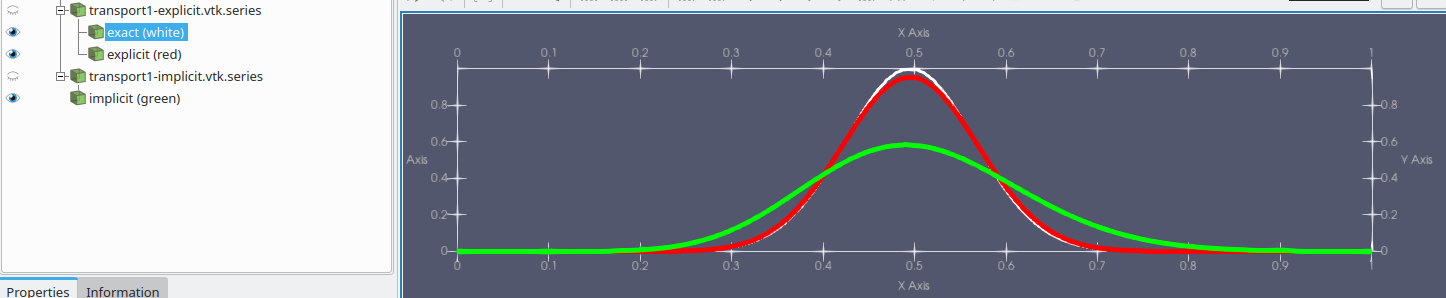
\includegraphics[width=1.0\linewidth]{transport1_solution.png}
\caption{Сравнение точного (белая линия) решения и численных решений по явной (красная) и неявной (зелёная) схемам}
\label{fig:transport1_solution}
\end{figure}

Чтобы получить такую картинку необходимо открыть в
Paraview сгенерированные в результате работы программ
выходные файлы \ename{transport1_explicit.vtk.series}
и \ename{transport1_implicit.vtk.series}
И далее проделать преобразования, описанные в пункте \ref{sec:paraview-1d}.

Для построения графиков сходимости, необходимо преобразовать
написанные программы, запустив цикл по различным значениям числа Куранта
\begin{minted}[linenos=false]{c++}
for (double Cu: { ... }){
    // solution
    ...

    std::cout << 1.0/tau << " " << norm << std::endl;
}
\end{minted}
и построить график полученной таблицы в логарифмических осях.
При задании диапазона изменений $C$ следует учитывать, что явная схема устойчива только при $C \leq 1$,
в то время как две другие схемы безусловно устойчивы.

Графики сходимости с уменьшением шага по времени
представлены на \figref{fig:transport1_norms}.

\begin{figure}[h]
\centering
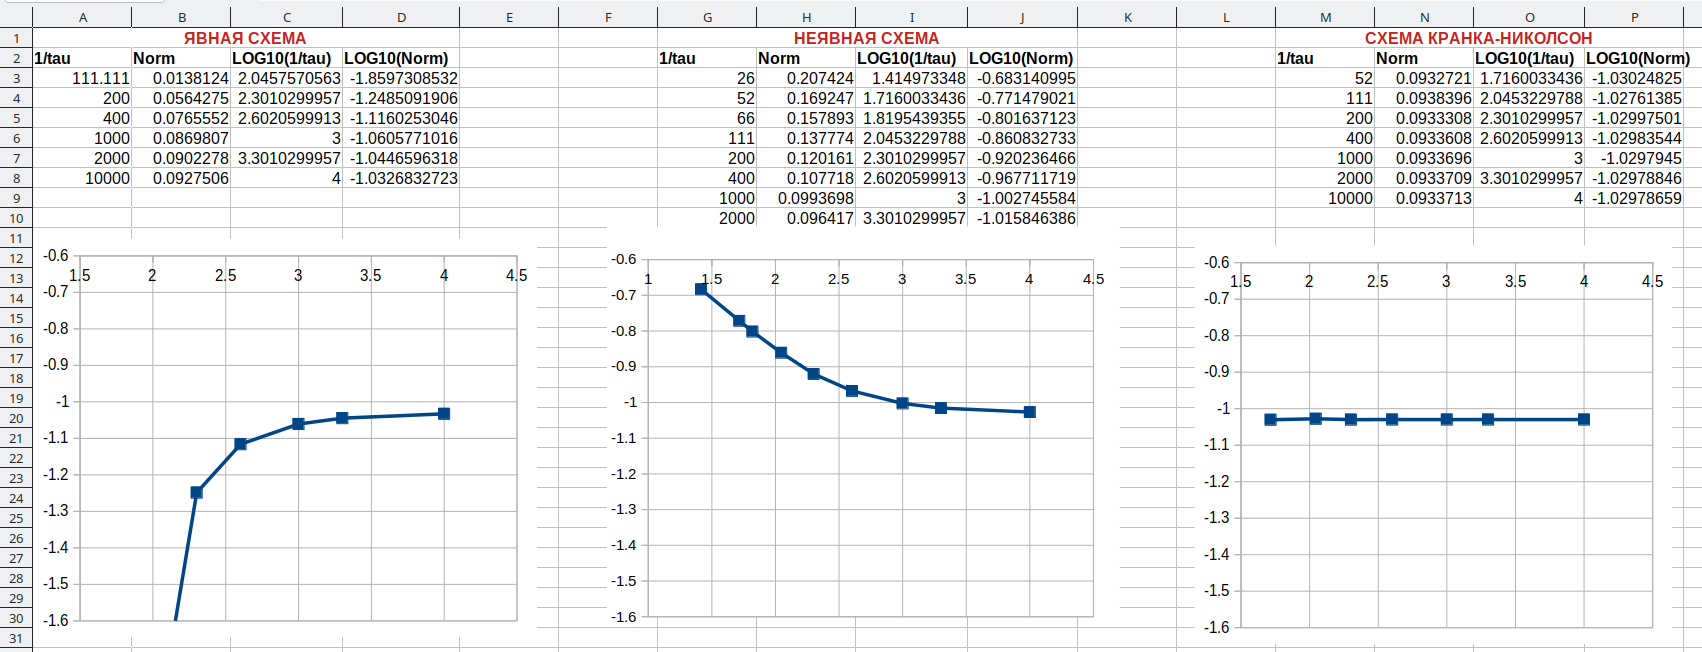
\includegraphics[width=1.0\linewidth]{transport1_norms.png}
\caption{Сходимость решения уравнения переноса с уменьшением $\tau$}
\label{fig:transport1_norms}
\end{figure}

Видно, что для явной схемы с уменьшением шага по времени
ответ отдаляется от точного, а для неявной -- наоборот, приближается.

Это объясняется тем, что в случае явной схемы
ошибки по времени и по пространству имеют разный знак
и (в случае их равенства) компенсируют друг друга.
А для неявной эти ошибки имеют одинаковый знак.

В пределе (с минимальным шагом по времени) все три схемы
сходятся к одной и той же ошибке (ошибке схемы по пространству).


\subsection{Задание для самостоятельной работы}
\subsubsection{Постановка задачи}
Написать двумерный решатель для уравнения переноса
\begin{equation*}
    \dfr{u}{t} + U \dfr{u}{x} + V \dfr{u}{y} = 0.
\end{equation*}

Решение проводить в квадрате $x,y\in[-1,1]$.

Требуется
\begin{itemize}
\item расчитать и нарисовать в Paraview нестационарное решение (см. \ref{sec:paraview-2d});
\item построить график, иллюстрирующий увеличение нормы ошибки
      с продвижением по времени;
\item исследовать устойчивость схемы. Эмпирическим путём выяснить,
      какое максимально возможный шаг по времени можно брать
      при фиксированном разбиении по пространству;
\item построить график, иллюстрирующий сходимость нормы
      ошибки при уменьшении шага по времени при фиксированном разбиении
      по пространству.
\end{itemize}

\subsubsubsection{Тестовый пример 1}
На этапе первичного тестирования использовать
значения скорости
\begin{equation*}
    U = 1, \quad V = 0.
\end{equation*}

А в качестве начального решения брать простой "столбик" (\figref{fig:transport1_work_01})
\begin{equation*}
    u(x,y,0) = u_0(x, y) = \begin{cases}
        1, & \; -1\leq x \leq -0.8, \; -0.1 \leq y \leq 0.1, \\
        0, & \; \text{иначе}.
    \end{cases}
\end{equation*}

\begin{figure}[h]
\centering
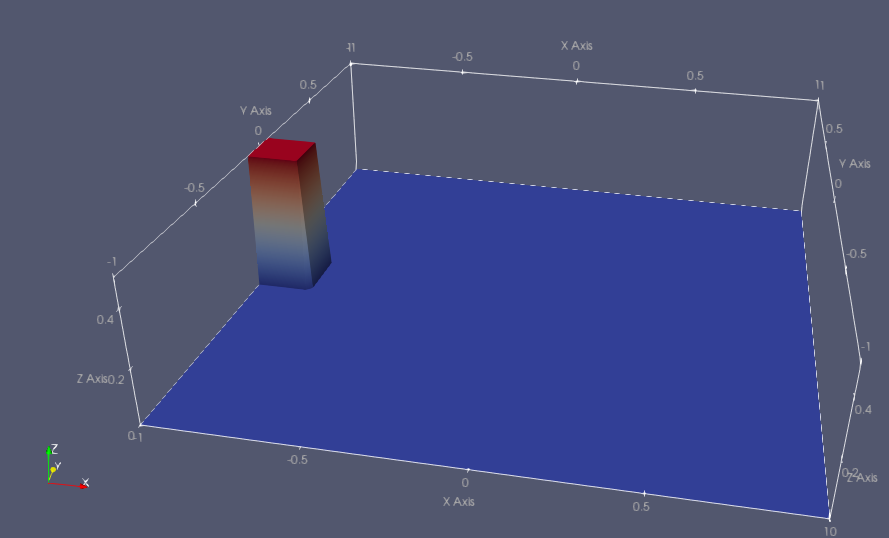
\includegraphics[width=1.0\linewidth]{transport1_work_01.png}
\caption{Начальные условия для первого тестового примера}
\label{fig:transport1_work_01}
\end{figure}

Точным решением будет функция
\begin{equation*}
    u^e(x, y, t) = u_0(x-t, y)
\end{equation*}

То есть этот столбик будет двигаться вправо с единичной
скоростью и за время 2 полностью покинет расчётную область.

\subsubsubsection{Тестовый пример 2}

После того, как этот тест будет пройден,
использовать постановку с непостоянной по пространству скоростью
\begin{equation*}
    U(x, y) = -y, \quad V(x, y) = x.
\end{equation*}

и начальным решением вида (\figref{fig:transport1_work_02})
\begin{align*}
    &r_0(x, y) = \sqrt{(x - 0.5)^2 + y^2}; \; \sigma = 0.1;\\
    &u(x, y, 0) = u_0(x, y) = e^{-r_0^2(x, y)/\sigma^2}
\end{align*}

\begin{figure}[h]
\centering
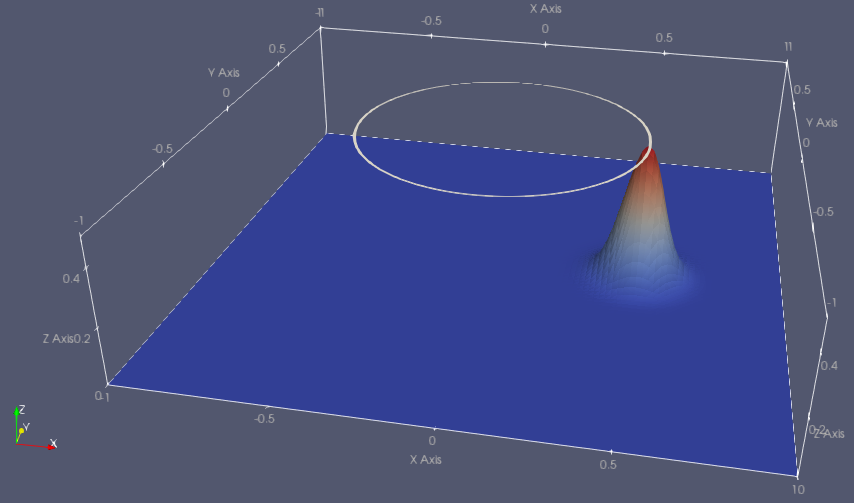
\includegraphics[width=1.0\linewidth]{transport1_work_02.png}
\caption{Начальные условия для второго тестового примера}
\label{fig:transport1_work_02}
\end{figure}

В процессе решения этот "холмик" будет
двигаться по окружности, описывая полный оборот за время $t=4\pi$.

Точное решение на момент времени $t$ будет иметь вид
\begin{align*}
  	& x_c(t) =  0.5\cos(0.5 t); \\
    & y_c(t) =  0.5\sin(0.5 t); \\
    & r(x, y, t) = \sqrt{(x - x_c(t))^2 + (y - y_c(t))^2};  \\
    & u^e(x, y, t) = e^{-r^2(x, y, t)/\sigma^2}
\end{align*}


\subsubsection{Расчётная схема}

Использовать противопотоковую явную схему:
\begin{equation*}
    \frac{\hat u_k - u_k}{\tau}
        + |U_k| \frac{u_k - u_{\upx{k}}}{h_x}
        + |V_k| \frac{u_k - u_{\upy{k}}}{h_y} = 0
\end{equation*}

Здесь $\upx{k}$, $\upy{k}$ -- 
значения индексов, расположенных против потока
отностительно узла $k$ в направлениях $x$ и $y$ соответственно.

Поскольку скорость в настоящей постановке непостоянная и зависит от точки пространства,
то вычислять индекс узла, расположенного против потока
приходится в зависимости от значения скорости.
С использованием ранее введёных алгоритмов перехода
от парных (i, j) индексов к сквозному индексу $k$ \eqref{eq:tasks_ij2k} и обратно \eqref{eq:tasks_k2ij} запишем
\begin{align*}
    & i = i[k]; \\
    & j = j[k]; \\
    & \upx{k} = \begin{cases}
          k[i-1, j], & \quad U_k \geq 0, \\
          k[i+1, j], & \quad U_k < 0 ,\\
      \end{cases} \\
    & \upy{k} = \begin{cases}
          k[i, j-1], & \quad V_k \geq 0, \\
          k[i, j+1], & \quad V_k < 0.\\
      \end{cases}
\end{align*}

В схеме скорости переноса взяты по абсолютному значению.
Это связано с зависимостью направления конечной разности от знака скорости.
Так если $U_k > 0$, то для дискретизации производной по $x$ используется разность
назад:
\begin{equation*}
    U\dfr{u}{x} \approx U_k\frac{u_{k[i, j]} - u_{k[i-1, j]}}{h_x}
    = |U_k|\frac{u_{k[i, j]} - u_{k[i-1, j]}}{h_x}
    = |U_k|\frac{u_{k[i, j]} - u_\upx{k}}{h_x}
\end{equation*}
Если же $U_k < 0$, то используется разность вперёд
\begin{equation*}
    U\dfr{u}{x} \approx U_k\frac{u_{k[i+1, j]} - u_{k[i, j]}}{h_x}
    = -U_k\frac{u_{k[i, j]} - u_{k[i+1, j]}}{h_x} 
    = |U_k|\frac{u_{k[i, j]} - u_{k[i+1, j]}}{h_x} 
    = |U_k|\frac{u_{k[i, j]} - u_\upx{k}}{h_x} 
\end{equation*}

На границах использовать условия первого рода. Можно просто нули, поскольку они соответствуют постановке.
